\section{Introduction à l'Intelligence Artificielle (IA)}

Cette section se base sur la documentation fournie par DataCamp \cite{datacamp} et explore le vaste domaine de l'intelligence artificielle. L'intelligence artificielle est un domaine vaste qui vise à permettre aux machines d'imiter le comportement humain. Il comprend plusieurs branches, dont l'apprentissage automatique, qui permet à une machine ou un système d'apprendre ou de s'améliorer sans ou avec très peu d'intervention humaine. On distingue généralement trois approches de l'apprentissage automatique : l'apprentissage supervisé, l'apprentissage non supervisé et l'apprentissage par renforcement. \\

\noindent Dans l'apprentissage supervisé, un modèle est entraîné à partir d'un ensemble de données étiquetées, tandis que dans l'apprentissage non supervisé, le modèle doit découvrir par lui-même des structures ou des relations dans des données non étiquetées. Dans l'apprentissage par renforcement, le modèle reçoit des récompenses ou des pénalités en fonction des décisions qu'il prend. \\


\noindent Pour notre étude, nous allons nous focaliser sur une sous-branche de l'apprentissage automatique, connue sous le nom d'apprentissage profond et plus précisement l'apprentissage par réseau de neurones. Cette approche permet aux systèmes informatiques d'imiter la structure et le fonctionnement des neurones humains, grâce à des réseaux de neurones artificiels. L'apprentissage profond est largement utilisé pour la classification et offre des capacités puissantes en matière de modélisation et de représentation des données complexes.

\subsection{Choix de la méthode d'IA}

L'apprentissage profond, comme mentionné précédemment, reproduit la structure et le fonctionnement des neurones humains à travers des neurones artificiels, afin de découvrir des relations complexes entre les données. En effet, les neurones biologiques sont constitués de dendrites et d'axones, qui reçoivent et émettent des signaux, correspondant respectivement à l'entrée et à la sortie du neurone. Ces concepts sont modélisés par des entrées et des sorties dans les modèles de neurones artificiels. La Figure 13 présente une comparaison entre un neurone biologique et la forme la plus simple d'un réseau de neurones, le perceptron. \\

\begin{figure}[H]
            \centering
           \fbox{ 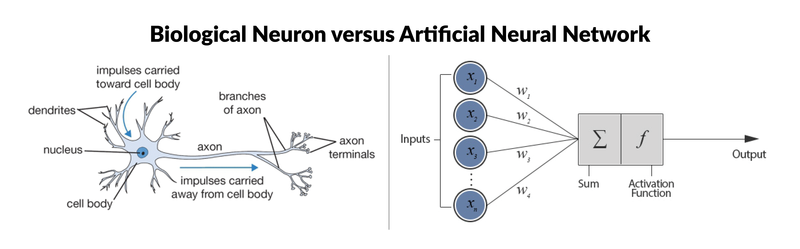
\includegraphics[width=15cm]{images/content_content_neuron.png}}   
            \caption{Comparaison d'un nerone avec un perceptron  -  \cite{datacamp}} 
        \end{figure}

\noindent Un perceptron peut être considéré comme une fonction mathématique qui prend en entrée un ensemble de données, effectue des opérations spécifiques, applique une fonction d'activation pour réguler les valeurs dans un intervalle selon la fonction choisie, et produit ensuite un résultat en sortie. \\

\begin{equation}
\hat{y} = \sigma(\sum_{x \in X } x \theta )
\label{moneq}
\end{equation} 
\vspace{1cm}

\noindent L'équation \eqref{moneq} entraîne plusieurs éléments, chacun ayant un rôle spécifique. La notation $\sum_{x \in X} x \theta$ représente la somme pondérée des entrées, où $x$ correspond aux différentes valeurs des caractéristiques de l'entrée, $\theta$ désigne les poids et biais associés à ces caractéristiques, et la sommation est effectuée sur l'ensemble des caractéristiques de l'entrée $X$. La fonction d'activation $\sigma$ est appliquée à la somme pondérée des entrées pour produire $\hat{y}$, qui représente la prédiction du modèle. \\

\noindent Les modèles basés sur un simple perceptron fonctionnent en classifiant les données en seulement deux classes à l'aide d'une limite tracée par une ligne droite, ce qui n'est pas adapté lorsque plusieurs classes sont présentes. Pour surmonter cette limitation, des modèles plus complexes existes. Elles sont constitués de différentes couches contenant un ensemble de perceptrons qui interagissent entre-eux pour extraire les caractéristiques essentielles des données en vue de leurs classifications. (\textit{cf.} Figure 13).\\


\begin{figure}[H]
            \centering
           \fbox{ 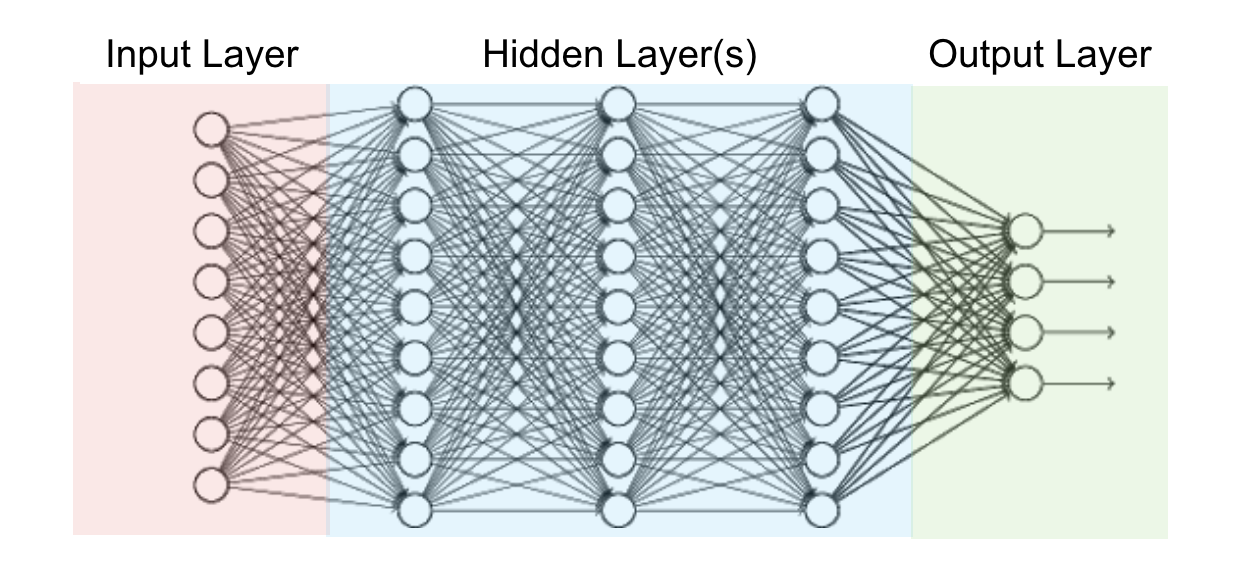
\includegraphics[width=12cm]{images/HiddenLayers.png}}   
            \caption{Illustration des diverses couches dans l'apprentissage profond -  \cite{hiddenlayer}} 
        \end{figure}


\noindent L'entraînement de nos données se déroulera sur des réseaux de convolution, exploitant la rétropropagation du gradient. Cette technique permet de mettre à jour les paramètres $\theta$ du modèle, afin de minimiser la fonction de coût.\\


\noindent La fonction de coût est généralement calculée comme la moyenne des fonctions de perte pour chaque exemple de données. Ces fonctions de perte mesurent la différence entre les valeurs réelles et les valeurs prédites par le modèle. En minimisant cette fonction de coût, l'objectif est d'améliorer les performances globales du modèle en termes de précision et de capacité de généralisation.\\

\noindent Cette approche permet aux réseaux de neurones profonds de capturer des caractéristiques complexes dans les données, ce qui les rend efficaces pour la classification et l'identification de données.



\subsection{Environnement de travail}

Cette section est inspirée des consignes fournies par le site de TensorFlow \cite{TensorFlow} pour configurer un environnement de travail afin d'exploiter pleinement la capacité du GPU et d'optimiser l'utilisation des modèles d'apprentissage profond. Étant donné que la dernière version de TensorFlow prenant en charge le GPU sur Windows natif est la version 2.10, nous avons choisi de configurer la version 2 du Windows Subsystem Linux qui permet de lancer des exécutables Linux sur Windows. Cette solution permet de profiter des versions plus récentes de TensorFlow. \\

\noindent De plus, nous avons configuré Visual Studio Code pour qu'il fonctionne correctement avec TensorFlow en utilisant le GPU. Nous avons ainsi suivi les étapes suivantes. \\

\begin{itemize}
    \item Nous avons installé et configuré Windows Subsystem for Linux version 2 (WSL2) sur mon système.
    \item Nous avons ensuite procédé à l'installation et à la configuration d'Ubuntu dans WSL2, créant ainsi un environnement Linux fonctionnel ;
    \item Nous avons installé la dernière version de TensorFlow compatible avec l'utilisation du GPU, afin de bénéficier de ses performances optimales ;
    \item Pour permettre à TensorFlow d'utiliser le GPU, Nous avons  installé les pilotes NVIDIA nécessaires pour CUDA.
Nous avons configuré Visual Studio Code pour exécuter le code dans le nouvel environnement Linux, assurant ainsi une intégration fluide avec mes projets TensorFlow ;
    \item Enfin, Nous avons vérifié que le GPU était correctement configuré et utilisé par TensorFlow, ce qui nous a permis d'exécuter nos codes et nos modèles sur le GPU avec succès.
\end{itemize}

\subsection{Conclusion}

En conclusion, l'intégration de l'intelligence artificielle, notamment à travers l'apprentissage profond et la configuration de l'environnement de travail avec TensorFlow sur un GPU, sont bénéfique pour traiter les données complexes obtenues des capteurs d'Hyperion. Les réseaux de neurones sont capables d'analyser les relations complexes de ces données et d'extraire des informations cruciales pour les identifier, même lorsque celles-ci ne sont pas visibles à premiere vue. D'autre part, la configuration du GPU accélère le processus d'apprentissage des modèles, permettant ainsi d'économiser du temps. Ensembles, ces technologies permettent d'identifier les traverses et la topologie de façon plus précise et rapide.



